\documentclass{article}

\usepackage{xeCJK}
% 段落缩进
\usepackage{indentfirst}
% 参考文献
\bibliographystyle{alpha}
% 索引
\usepackage{makeidx}
\makeindex
% 图片
\usepackage{graphicx}
% 标题
\usepackage{caption}
\captionsetup{figurename=图, tablename=表}
% 页面尺寸
\usepackage{geometry}
\geometry{a4paper, left=2cm, right=4cm, top=2cm, bottom=2cm}

\title{利用开源软件\\搭建数据存储和处理基础设施的实践记录}
\author{周加根(zhoujiagen@gmail.com)}
%\date{2017-03-05}

% 在Mac应用>字体册.app中查看
\setCJKmainfont{Lantinghei SC Extralight}
\begin{document}
% 段落间距
\setlength{\parskip}{0.5em}
\maketitle

\renewcommand\abstractname{简述}
\begin{abstract}
% 段落间距
\setlength{\parskip}{0.5em}
两年之前想在语义网方向做一点延伸探究工作, 即搭建SPARQL端点之外的三元组(Triple)的存储和处理实验环境. 在考察Apache Jena的过程中, 发现了其Apache Jena Elephant子项目, 该项目在Apache Hadoop的基础上处理Triple, 但所提供的处理方法较少, 开发进展缓慢.

尽管当前纯粹语义网技术的应用已见少, 但在自然语言处理(NLP)、机器学习技术和基于知识图谱的推理的助力下, 仍存在大量可做的工作. 包括大规模Triple存储、从纯粹的建模表征性视角转变为向量等统计推断算法操作性视角等等.

基于上述的观察, 一方面需要准备具备能力的数据管理基础设施, 另一方面需要准备恰当的数学理论工具. 本文作为考察开源软件搭建数据管理基础设施的记录, 主要关注于既有大规模数据存储和处理的实践, 以期为后续数据理论工具的应用做好准备.

在记录特定开源软件时, 尝试从核心抽象、工作机制和应用案例三个角度进行阐述.

\end{abstract}

\newpage

\renewcommand\contentsname{目录}
\tableofcontents

\newpage

\section{Apache Hadoop}

Hadoop起源于Apache Nutch项目, 由Doug Cutting创建, 于2008年成为Apache顶级项目. 其实现过程中参考了Google的工作\cite{GFS} 、\cite{MapReduce}.
\index{Hadoop}

Hadoop提供了在简单编程模型下跨集群的大数据集的分布式处理能力, 同时提供了在应用层检测和处理失败的高可用服务保证. 项目由四个主要模块构成:

\begin{enumerate}
\item[(1)] Hadoop Common\\
支持其他模块的公用工具.
\item[(2)] Hadoop Distributed File System(HDFS)\\
提供高吞吐量应用数据访问的分布式文件文件系统.
\item[(3)] Hadoop YARN\\
作业调度和集群资源管理的框架.
\item[(4)] Hadoop MapReduce\\
基于YARN的大数据集并行处理系统.
\end{enumerate}

下文的阐述主要参考了\cite{hadoop-defnitive-guide}.

\subsection{核心抽象}

\subsubsection{HDFS}

作为GFS\cite{GFS}的开源实现, HDFS提供了在普通机器上搭建可扩展的可容错的分布式文件系统实现. 
\index{GFS} \index{HDFS}

HDFS的设计权衡是大多数数据处理模式是\textbf{write-once read-many-times}, 设计为不支持低延迟的数据访问, 同时为加快数据查找而尽量的将文件系统的元数据放在内存中而不支持大量的小文件. HDFS的另一设计权衡是承认失效总是存在的, 数据的持久性依赖依赖于冗余的存储副本.

同单块磁盘上一次可读写的磁盘块概念类似, HDFS中也存在通常默认为128M的块(block). 典型的HDFS集群由两类节点按master-slave工作模式构成: 作为master的namenode和作为worker的datanode. namenode管理文件系统的命名空间, 包括文件系统树、树中文件和目录的元信息. datanode按namenode或者客户端的要求存储和查找文件块, 并定期向namenode报告其存储的文件块信息.
\index{Master-slave pattern}
\index{namenode}
\index{datanode}

HDFS中文件读取步骤见图\ref{fig:hdfs-read-data}:

\begin{enumerate}
\item[(1)] 客户端通过调用\texttt{FileSystem.open()}打开文件, 在HDFS中调用\texttt{DistirbutedFileSystem};
\item[(2)] \texttt{DistirbutedFileSystem}使用远程过程调用(Remote Procedure Call, RPC)询问namenode, 定位文件中第一个块的位置. 对每个块, namenode返回有该块副本的所有datanode的位置;

\texttt{DistirbutedFileSystem}返回\texttt{FSDataInputStream}给客户端, 客户端可以从该流中读取数据. \texttt{FSDataInputStream}封装了管理datanode和namenode I/O的\texttt{DFSInputStream}.

\index{RPC}
\index{DistirbutedFileSystem}
\index{FSDataInputStream}
\index{DFSInputStream}

\item[(3)] 客户端调用\texttt{FSDataInputStream.open()}, \texttt{DFSInputStream}中已经有文件第一个块所在的datanode位置信息, 它连接到最近的datanode获取文件第一个块;
\item[(4)] 客户端调用\texttt{FSDataInputStream.read()}读取文件第一个块中数据;
\item[(5)] 读到文件块尾部时, \texttt{DFSInputStream}关闭与datanode的连接, 查找下一个块所在的datanode. 这对客户端是透明的, 从客户端的视角看是在读取连续的流. 这一步骤中\texttt{DFSInputStream}会在需要时访问namenode以获取下一批文件块的datanode位置;
\item[(6)] 客户端读取完数据时, 调用\texttt{FSDataInputStream.close()}关闭流.
\end{enumerate}

\begin{figure}
\centering
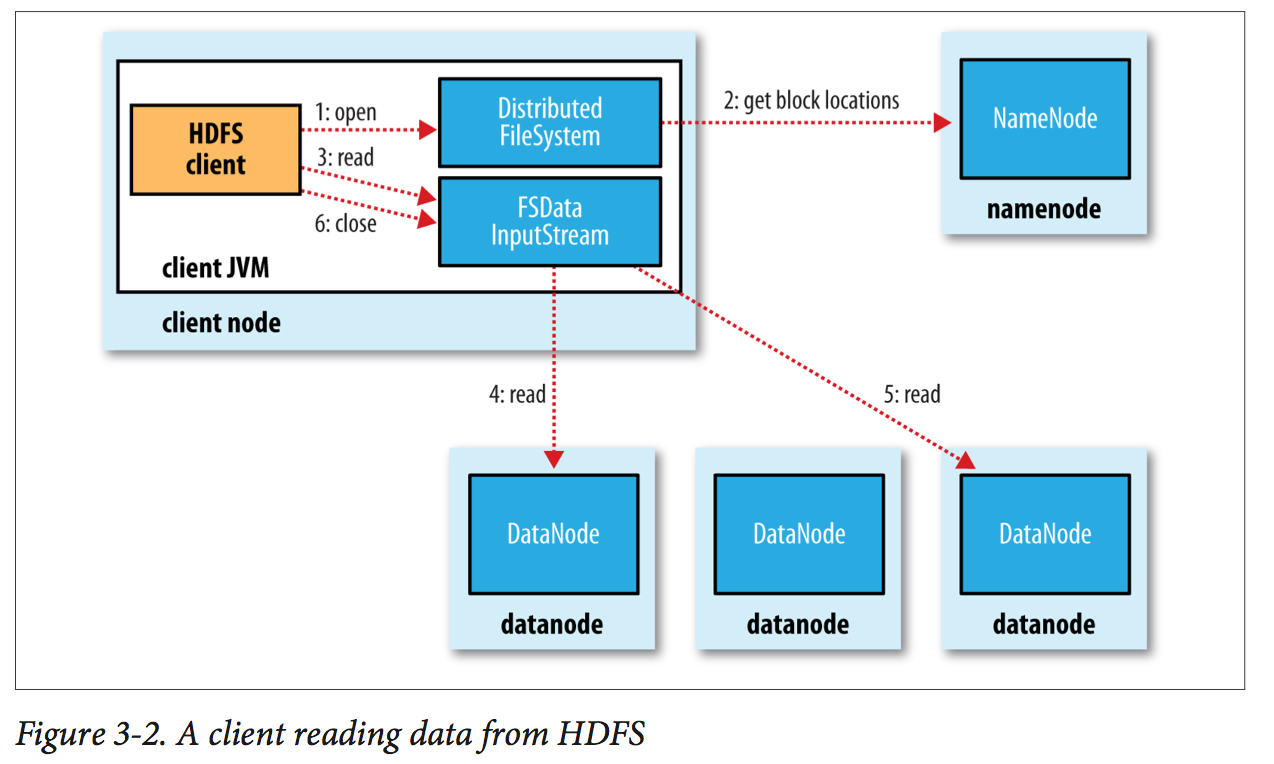
\includegraphics[scale=0.5]{image/hdfs-read-data.png}
\caption{HDFS数据读取}\label{fig:hdfs-read-data}
\end{figure}

HDFS中文件写入步骤见图\ref{fig:hdfs-write-data}:

\begin{figure}
\centering
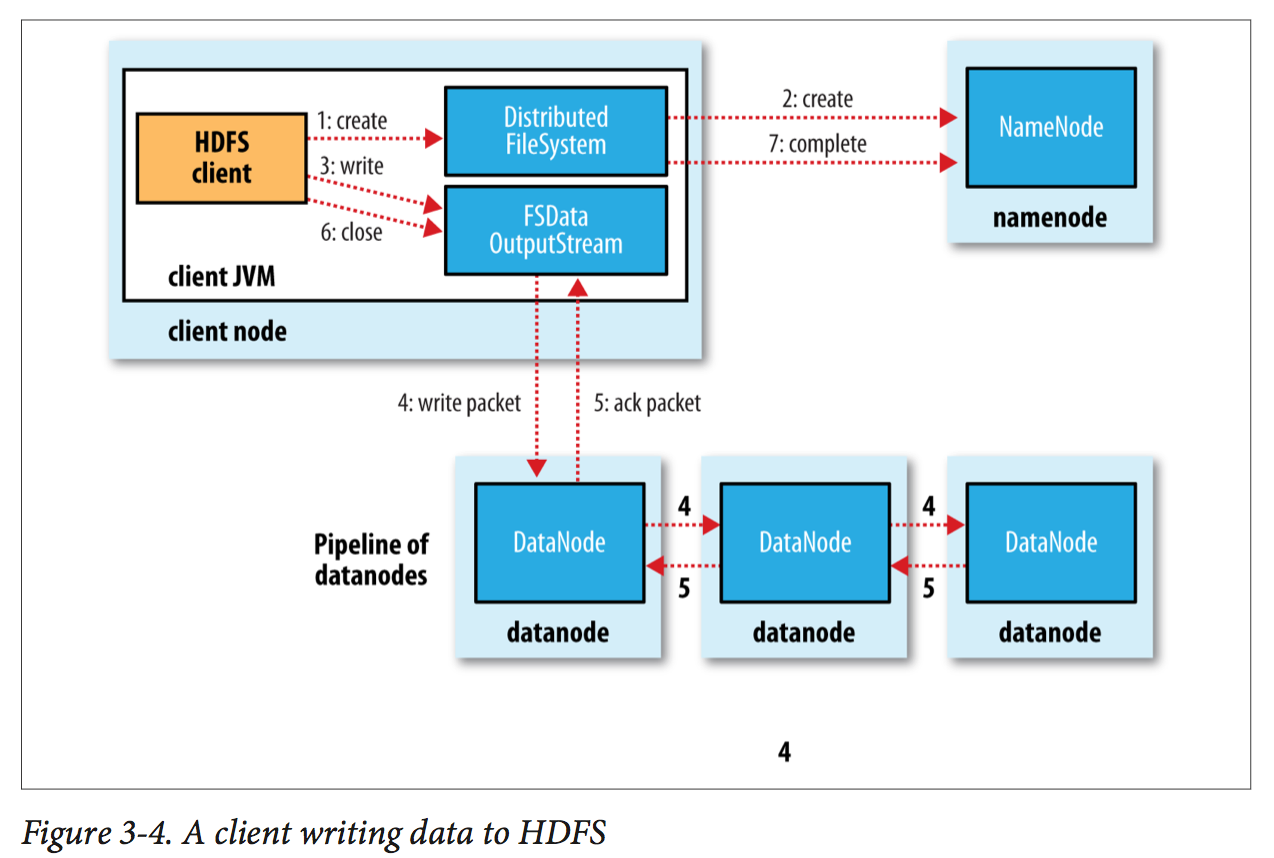
\includegraphics[scale=0.5]{image/hdfs-write-data.png}
\caption{HDFS数据写入}\label{fig:hdfs-write-data}
\end{figure}

\subsubsection{MapReduce}

\subsubsection{IO格式}

SubSection content.

\subsection{工作机制}

\subsection{应用案例}

\subsection{相关概念}

\newpage


\newpage
\renewcommand\refname{参考文献}
\bibliography{references}

\newpage
\renewcommand\indexname{索引}
\printindex

\end{document}
